\chapter{Prova de Conceito}
Para validar o projeto final, foi proposta uma prova de conceito que aplica as tecnologias mencionadas para obter uma estimativa de distância a partir do Bluetooth.
No projeto final algoritmos, e técnicas mais elaboradas serão utilizados para uma maior precisão, porém na prova de conceito, é possível validar o projeto e mostrar os potenciais de atingir o objetivo final do projeto.

A seguir um detalhamento de como foi elaborada a prova de conceitos e os resultados atingidos.

\section{Hardware}
O Hardware escolhido para prova de conceito é a placa de desenvolvimento nRF52840 DK da fabricante de componentes Nordic Semiconductor \cite{nRF52840_site}.

Tal placa de desenvolvimento conta com o SoC nRF52840 que possui Bluetooth 5.0 integrado, e pinos de GPIO com entrada analógica, além de um amplo suporte de recursos online para o desenvolvimento. Soma-se a isso, sua compatibilidade com o SoC nRF52811 da mesma fabricante, que é um dos unicos chips atualmente que possui Bluetooth 5.1 e planeja-se utilizar na etapa final do projeto \cite{nRF52811_site}.

Como o nRF52840 DK não possui suporte para AoA, e placas de desenvolvimento do nRF52811 serão disponibilizadas somente no próximo semestre pela Nordic Semiconductor, pretende-se utilizar um interferômetro de 6-portas desenvolvido no departamento de sistemas eletrônicos da escola politécnica da USP para estimar o ângulo de chegada.

O interferômetro possuí 4 saídas analógicas. Fazendo-se a leitura dessas 4 saídas e utilizando a equação \ref{eq:eq_AoA} encontra-se o AoA.

\begin{figure}[H]
	\centering 
	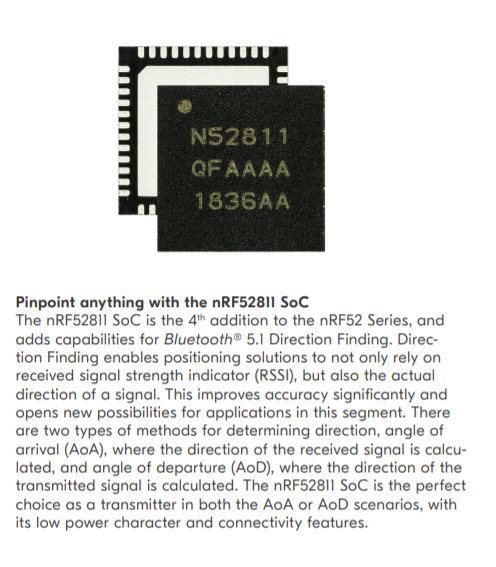
\includegraphics[scale = 1]{images/nRF52811.png}
	\caption{nRF52811. Tirado de \cite{nRF52811_site}}
	\label{fig:nRF52811}
\end{figure}


\begin{figure}[H]
	\centering 
	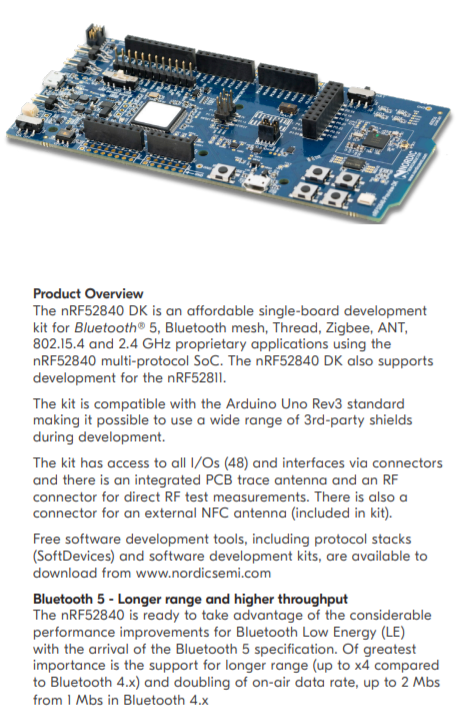
\includegraphics[scale = 1]{images/nRF52840_dk.png}
	\caption{nRF52840. Tirado de \cite{nRF52840_site}}
	\label{fig:nRF52840_dk}
\end{figure}


\section{Programa}
A placa de desenvolvimento, na prova de conceito foi programada para procurar dispositivos Bluetooth nas proximidades que tivessem um determinado ID no pacote de \textit{advertising}. Caso fosse encontrado, cada instante que houvesse uma mudança de mais de 5dbm na intensidade do sinal, este era imprimido em uma porta serial.

Além disso, utilizou-se a equação \ref{eq:rssi} para estimar a distância do sinal recebido. O valor para o fator de perda utilizado foi de \(n = 4\) e adotou-se o valor de \(A = -45dbm\).

O dispositivo que emitia o sinal Bluetooth a ser lido foi um celular Samsung Galaxy S8 com Bluetooth 5.0 e um aplicativo pronto que permitia a configuração de um ID específico para um \textit{advertising} a ser enviado.

No programa, o ângulo de chegada ainda não foi implementado

\begin{figure}[H]
	\centering 
	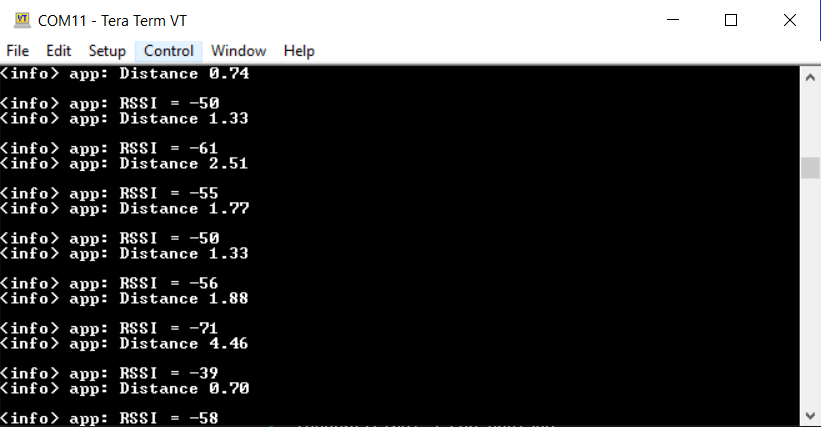
\includegraphics[scale = 0.85]{images/rssi_terminal.png}
	\caption{Porta serial do nRF52840 imprimindo valores de RSSI recebidos}
	\label{fig:rssi_terminal}
\end{figure}

\section{Arranjo Experimental}
O arranjo experimental, consistiu em fazer medições de distâncias reais de 0.5m em 0.5m em um ambiente fechado e compará-las com as distâncias estimadas pelos programas e hardware descritos, como se observa na seguinte figura:

\begin{figure}[H]
	\centering 
	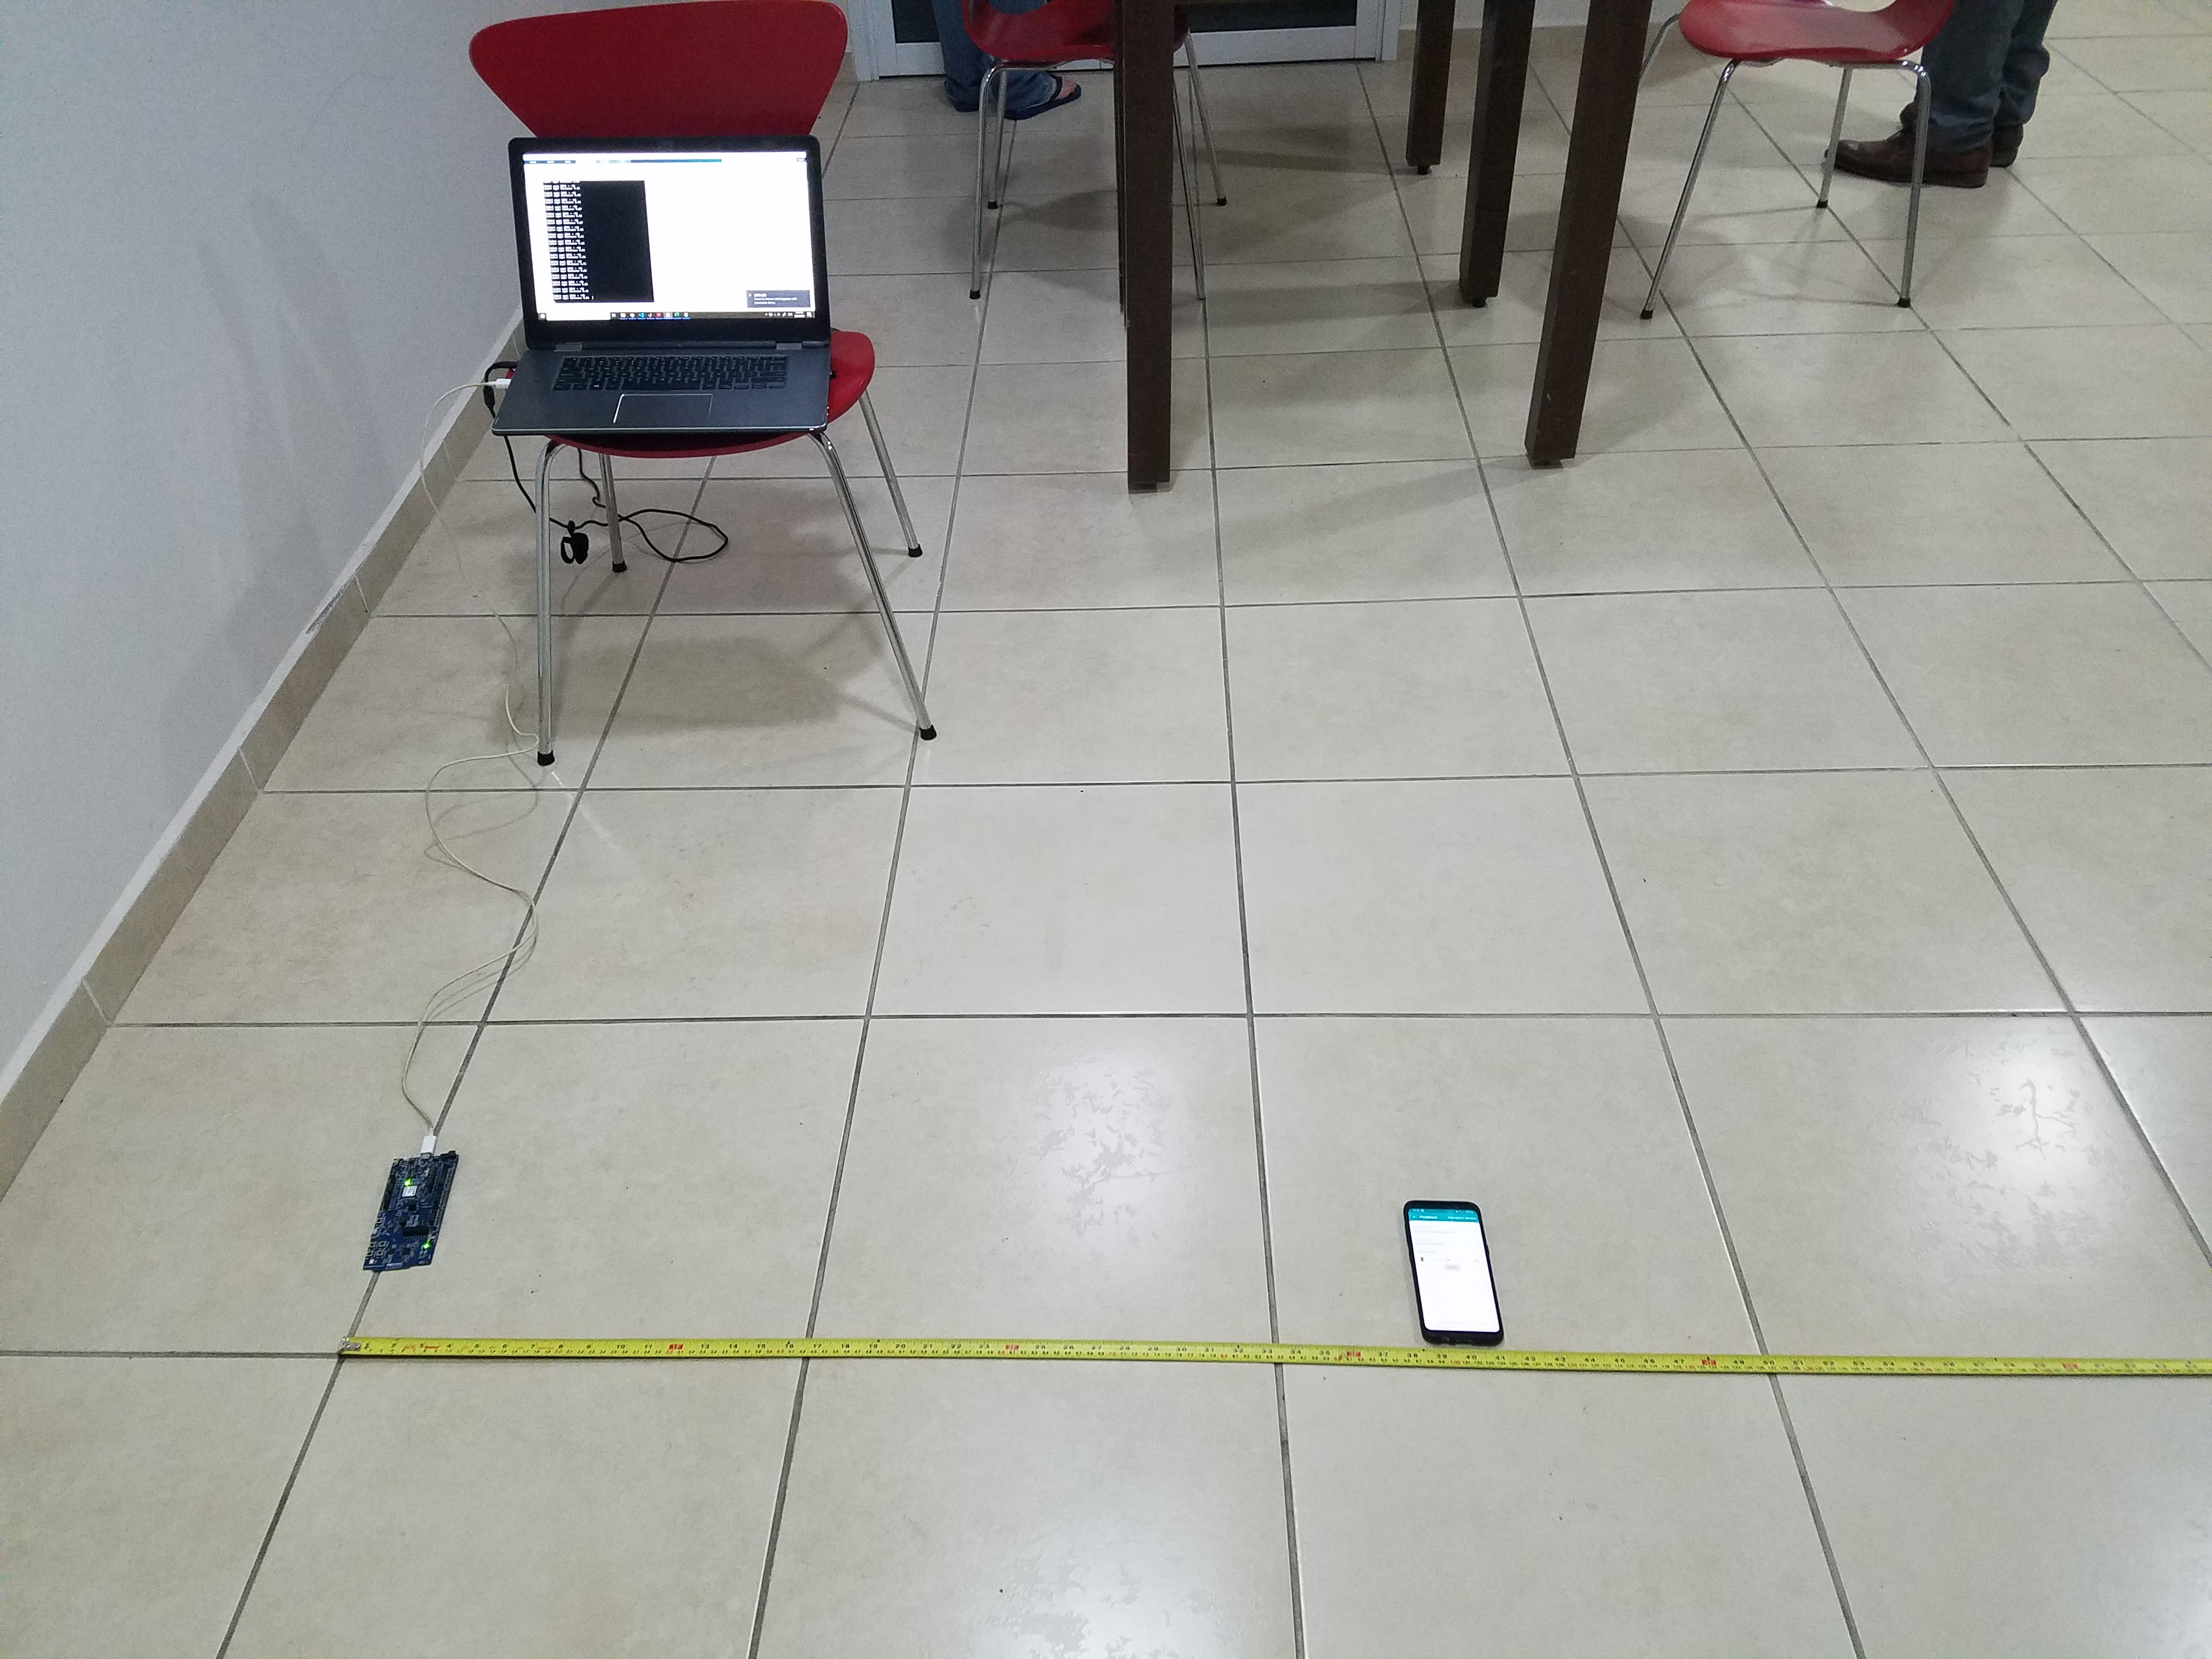
\includegraphics[scale = 0.1]{images/setup_poc.jpg}
	\caption{Arranjo experimental da prova de conceito}
	\label{fig:setup_poc}
\end{figure}


\section{Resultados}

Com os dados obtidos, foi possível construir os seguintes gráficos que evidenciam a precisão obtida.
Nota-se que a distância estimada é uma média de 10 leituras diferentes do celular na mesma posição.

\begin{figure}[H]
	\centering 
	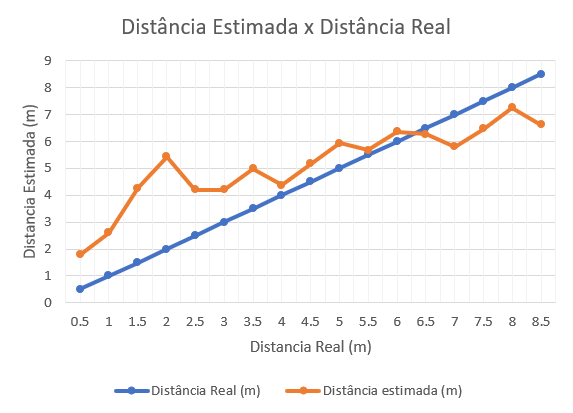
\includegraphics[scale = 1]{images/grafico_distancias_1d.png}
	\caption{Distância Estimada x distância real na prova de conceito}
	\label{fig:grafico_distancia_1d}
\end{figure}

\begin{figure}[H]
	\centering 
	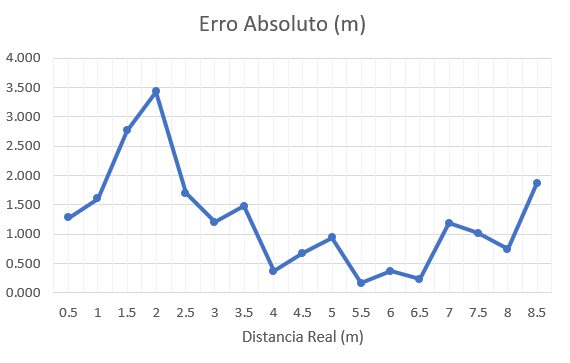
\includegraphics[scale = 1]{images/grafico_erro_1d.png}
	\caption{Erro absoluto em metros em cada distância}
	\label{fig:grafico_erro_1d}
\end{figure}

Deste modo, pelos gráficos apresentados, nota-se que a precisão fica na ordem de 1m a 10m. Tais resultados foram obtidos com o algoritmo mais direto possível e somente utilizando a intensidade do sinal recebido. Ao se introduzir algoritmos mais robustos, a exemplo dos que usam \textit{fingerprint} e AoA, a precisão encontrada será ainda maior.

Ainda como prova de conceito. Simulou-se um sistema de localização 2D utilizando-se somente RSSI e as medidas obtidas anteriormente de distância linear.
Estimou-se uma distância de 5m entre placas, sendo que a placa 1 está na coordenada (0,0) e a placa dois na coordenada (5,0).
Fazendo-se simplificações para o caso 2D na equação \ref{eq:rssi} e substituindo-se os valores, as equações para obter coordenadas em tal sistema são:

\begin{equation}
    x = \frac{a^2 - b^2 + 25}{10} 
\end{equation}
\begin{equation}
    y = \sqrt{a^2 - x^2}
\end{equation}

Em que \(a\) é a distância para a placa na posição (0,0) e \(b\) a distância para a placa da posição (0,5).

Os resultados obtidos a partir disso foram:

\begin{center}
    \begin{tabular}{||c c c c c c c c c||} 
    \hline
    a Real 1 & b Real 2 & a 1 & b 2 & x Calc & y Calc	& x Real & y Real & Erro\\ [0.5ex] 
    \hline\hline
    1 & 5 & 2.61 & 5.94 & -0.34 & 2.58 & 0.10 & 0.99 & 1.64\\ 
    \hline
    2 & 5 & 5.43 & 5.94 & 1.92 & 5.07 & 0.40 & 1.95 & 3.47\\ 
    \hline
    3 & 2.5 & 4.21 & 4.20 & 2.50 & 3.38 & 2.77 & 1.15 & 2.24\\ 
    \hline
    3 & 5 & 4.21 & 5.94 & 0.74 & 4.14 & 0.90 & 2.86 & 1.29\\ 
    \hline
    3 & 7.5 & 4.21 & 6.48 & 0.07 & 4.20 & -2.22 & 2.01 & 3.16\\ 
    \hline
    4 & 1 & 4.37 & 2.61 & 3.72 & 2.29 & 4.00 & 0.00 & 2.30\\ 
    \hline
    4 & 2.5 & 4.37 & 4.20 & 2.64 & 3.48 & 3.47 & 1.98 & 1.71\\ 
    \hline
    4 & 5 & 4.37 & 5.94 & 0.88 & 4.27 & 1.60 & 3.66 & 0.94\\ 
    \hline
    4 & 7.5 & 4.37 & 6.48 & 0.20 & 4.36 & -1.52 & 3.69 & 1.84\\ 
    \hline
    5 & 1 & 5.94 & 2.61 & 5.34 & 2.60 & 4.90 & 0.99 & 1.66\\ 
    \hline
    5 & 2.5 & 5.94 & 4.20 & 4.26 & 4.14 & 4.37 & 2.42 & 1.72\\ 
    \hline
    5 & 5 & 5.94 & 5.94 & 2.50 & 5.38 & 2.50 & 4.33 & 1.05\\ 
    \hline
    5 & 7.5 & 5.94 & 6.48 & 1.82 & 5.65 & -0.62 & 4.96 & 2.53\\ 
    \hline
    6 & 1 & 6.37 & 2.61 & 5.87 & 2.47 & 6.00 & 0.00 & 2.47\\ 
    \hline
    6 & 2.5 & 6.37 & 4.20 & 4.79 & 4.19 & 5.47 & 2.46 & 1.85\\ 
    \hline
    6 & 5 & 6.37 & 5.94 & 3.02 & 5.60 & 3.60 & 4.80 & 0.98\\ 
    \hline
    6 & 7.5 & 6.37 & 6.48 & 2.35 & 5.92 & 0.47 & 5.98 & 1.88\\ 
    \hline
    7 & 2.5 & 5.81 & 4.20 & 4.11 & 4.10 & 6.77 & 1.77 & 3.53\\ 
    \hline
    7 & 5 & 5.81 & 5.94 & 2.34 & 5.31 & 4.90 & 4.99 & 2.57\\ 
    \hline
    7 & 7.5 & 5.81 & 6.48 & 1.67 & 5.56 & 1.77 & 6.77 & 1.21\\ 
    \hline
    8 & 5 & 7.25 & 5.94 & 4.22 & 5.89 & 6.40 & 4.80 & 2.43\\ 
    \hline
    8 & 7.5 & 7.25 & 6.48 & 3.55 & 6.32 & 3.27 & 7.30 & 1.01\\ [1ex] 
    \hline
   \end{tabular}
   \end{center}

   Da tabela, observa-se que mesmo no caso 2D os erros absolutos continuam na faixa de 1m a 10m utilizando-se somente o RSSI.